
\subsection{Crystal structure}

There are different ways a solid could arrange itself in order to fill a given volume and minimize the overall energy of the structure. One of the densest is the face-centered cubic (FCC) structure of for instance NaCl. Assuming a hard sphere model of atoms, the FCC has together with the hexagonal close packed (HCP) the theoretically highest density of any structure. The unit cell of FCC is cubic with volume $ V_{unitCell} = a^3 $ made up by a basis of 4 atoms. These are in positions $ a(0,0,0), \ a(0,0,\frac{1}{2}),\ a(0,\frac{1}{2}, 0)   $ and $ a(\frac{1}{2}, 0,0) $. Due to symmetry, each of these atoms are repeated throughout the structure, as illustrated in figure \ref{fig:fcc}. The corner atoms are  repetitions of the $ a(0,0,0)$ position, and each of these atoms are shared by 8 neighbouring cells. For the side atoms, they are shared only by two unit cells, giving at total of $ 6\cdot \frac{1}{2}=3 $ side atoms per unit cell and $ 8\cdot  \frac{1}{8}$ corner atoms in the unit cell. The density of a unit cell size given in lengths of Angstrom, the density of a FCC cell  is $\rho=  \frac{4}{a^3} \text{\AA}^{-3}$. 

\begin{figure}[H]
	\centering
	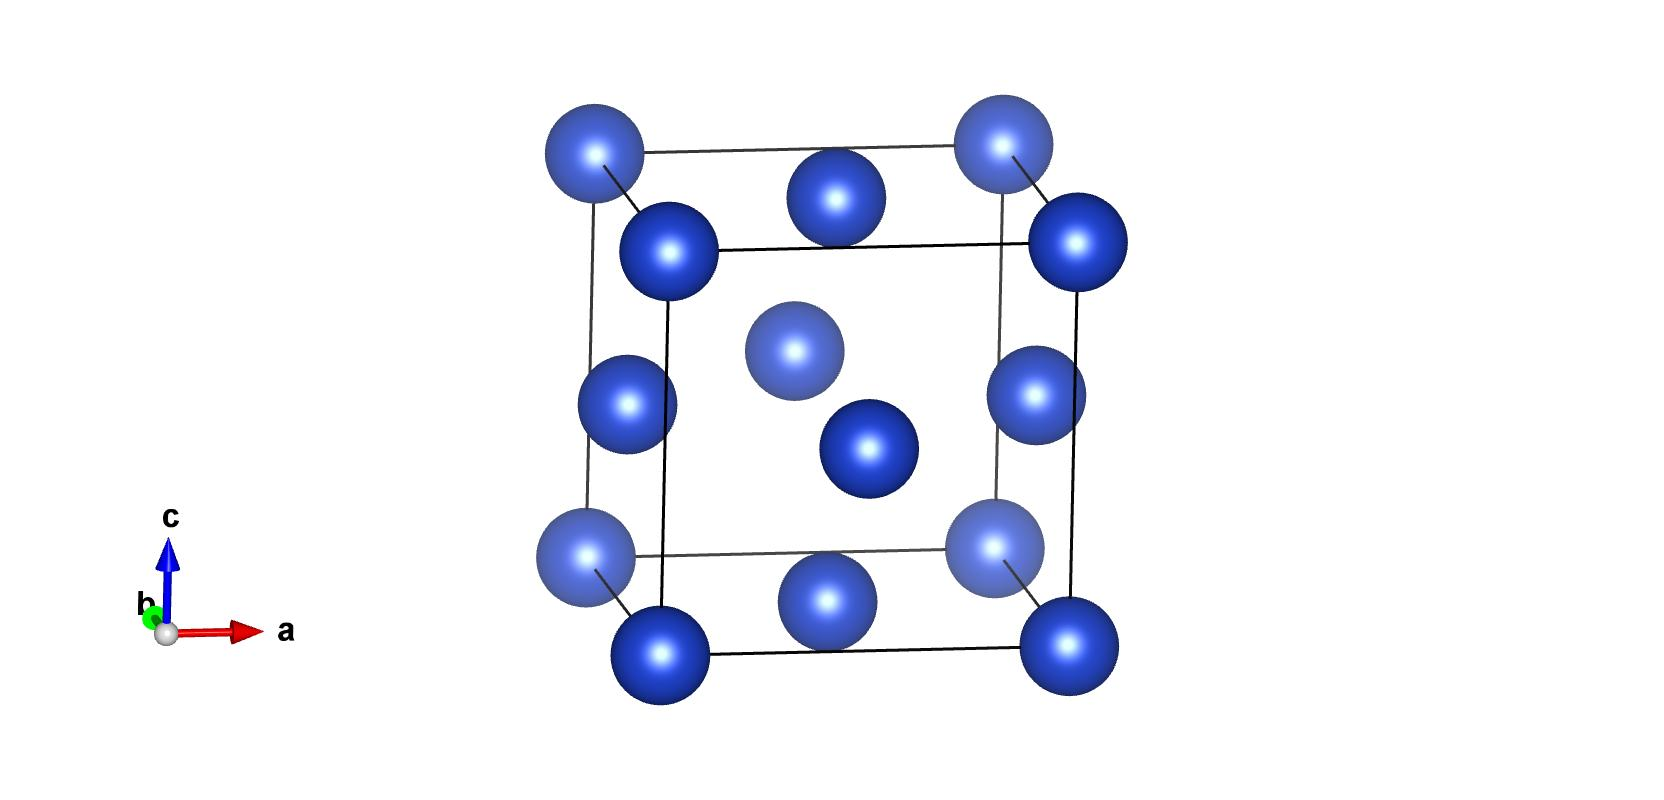
\includegraphics[width=0.7\linewidth]{../figures/fcc.jpg}
	\caption{Illustration of a fcc structure. Although there are 14 atoms in this figure, the unit cell is made up of 4 atoms. The rest of these appear because of symmetry.}
	\label{fig:fcc}
\end{figure}

In numerical calculations it is not possible to calculate on a infinite lattice of atoms. As an infinite lattice have neighbouring atoms in every direction for every atom, an atom can not move into vacuum. By applying periodic boundary conditions (PBC's) to the position of the lattice, every atom moving out of the predefined supercell is put on the other side of the box. In one dimension, this is expressed as $ r_{xi} = r_{xi}' - L $ if $ r_{xi} >L $, with $ L $ being the supercell size. This ensures that the density is constrained and the volume of the supercell remain constant. 

A surface experience different potential compared to bulk, as there are no neighbouring atoms in one of the directions, giving rise to different physics at the surface compared to the bulk. As infinite lattices does not have a surface, the surface effect needs to be minimized. By implementing the minimum image convention these effects can be reduced. This convention states that if a distance $ r_{ij} $ between two atoms $ i $ and $ j $ is larger than $ \frac{L}{2} $, the distance between them is $  r_{ij}'  = r_{ij}-L$. Thus an atom  near an edge experiences forces of approximately equal magnitude to an atom near the centre of the supercell. 

The PBC's and minimum image convention models an infinite supercell, by ignoring surface effects. However, it is not a true representation of an infinite cell. A perfect infinite cell consists of an infinite number of particles with random initial velocities, while a finite supercell will only have a finite number of atoms with sudorandom\footnote{If a computer is used to generate the random initial velocities. For the theoretical infinite lattice one usually assumes true random initial conditions} initial velocities. These atoms interact, leading to a stronger codependence of the neighbours for the finite case. By increasing the supercell this effect will decrease.   
 	
 

\subsection{Probability distribution}

v-distribution: why Mbolztmann
Discuss why the velocity of atoms are given from Maxwell-Boltzmann distrubution.  - nonzero net momentum. 




\subsection{Lennard Jones potential}

A very popular potential used in MD-simulations is the Lennard Jones potential, given in equation \ref{eq:LJ}. It describes the potential energy as a function of distance between two objects i and j, $ r_{ij} $. 

\begin{equation}\label{eq:LJ}
	U(r_{ij}) = 4\epsilon \left[	\left(\frac{\sigma}{r_{ij}}	\right)^{12}		- \left(\frac{\sigma}{r_{ij}}	\right)^{6}				\right]\\
\end{equation}

Through the relation $ 	F (\textbf{r} = -\nabla U(\textbf{r}) $, it is possible to determine the forces experienced by each atom by every other atom, simply as a function of the distance $ r_{ij} $ and relative position between two atoms. The distance $ r_{ij} $ is defined as  $ r_{ij}  = \abs{\textbf{r}_{ij}} = \abs{\textbf{r}_i - \textbf{r}_j} 	 $. By investigating each spatial direction separately, a relation for the forces between two atoms i and j arises: 

\begin{align}
		F_{ij}^x =& - \pdv{U}{r_{ij}} \pdv{r_{ij}}{x_{ij}}	\\	
		\pdv{r_{ij}}{x_{ij}} 		=& 		\dv{x_{ij}} \abs{\textbf{r}_i - \textbf{r}_j} 		=		 \dv{x_{ij}} \sqrt{ (\textbf{r}_i - \textbf{r}_j)^2}			\\
		 &= \frac{x_{ij}}{ \abs{\textbf{r}_i - \textbf{r}_j} } = \frac{x_{ij}}{r_{ij}}\\
		 \pdv{U}{r_{ij}} =& 4\epsilon \left[\frac{-12}{r_{ij}}\left(	\frac{\sigma}{r_{ij}}\right)^{12}		+  \frac{6}{r_{ij}} \left(\frac{\sigma}{r_{ij}}	\right)^{6}				\right]\\
		 F_x(r_{ij}) =& 24 \epsilon \left[		2	\left(\frac{\sigma}{r_{ij}}	\right)^{12}		- \left(\frac{\sigma}{r_{ij}}	\right)^{6}				\right] \frac{x_{ij}}{r_{ij}^2} \label{eq:Fx}
\end{align}

By generalising equation \ref{eq:Fx} to a three dimensional space one gets a general expression of the force between two atoms i and j: 
\begin{equation}\label{eq:F}
		  \textbf{F}(r_{ij}) = 24 \epsilon \left[		2	\left(\frac{\sigma}{r_{ij}}	\right)^{12}		- \left(\frac{\sigma}{r_{ij}}	\right)^{6}				\right] \frac{\textbf{r}_{ij}}{r_{ij}^2}
\end{equation}

Atom $ i $ experience a total force of $ F(\textbf{r}_i) =  \sum\limits_{j\neq i}   \textbf{F}(r_{ij})$. Each interaction is only necessary to compute once, as $ \textbf{r}_{ij}  = - \textbf{r}_{ji} $. However, it is necessary to update the force on each atom, according to Newtons third law. Equivalently, the total potential is given as $ U_{tot} =  \sum\limits_{i} \sum\limits_{j>i} 	U(\textbf{r}_{ij}) $. 



Potential surface????